\documentclass{report}

\documentclass[12pt]{article}
\usepackage{array}
\usepackage{color}
\usepackage{amsthm}
\usepackage{eufrak}
\usepackage{lipsum}
\usepackage{pifont}
\usepackage{yfonts}
\usepackage{amsmath}
\usepackage{amssymb}
\usepackage{ccfonts}
\usepackage{comment} \usepackage{amsfonts}
\usepackage{fancyhdr}
\usepackage{graphicx}
\usepackage{listings}
\usepackage{mathrsfs}
\usepackage{setspace}
\usepackage{textcomp}
\usepackage{blindtext}
\usepackage{enumerate}
\usepackage{microtype}
\usepackage{xfakebold}
\usepackage{kantlipsum}
%\usepackage{draftwatermark}
\usepackage[spanish]{babel}
\usepackage[margin=1.5cm, top=2cm, bottom=2cm]{geometry}
\usepackage[framemethod=tikz]{mdframed}
\usepackage[colorlinks=true,citecolor=blue,linkcolor=red,urlcolor=magenta]{hyperref}

%//////////////////////////////////////////////////////
% Watermark configuration
%//////////////////////////////////////////////////////
%\SetWatermarkScale{4}
%\SetWatermarkColor{black}
%\SetWatermarkLightness{0.95}
%\SetWatermarkText{\texttt{Watermark}}

%//////////////////////////////////////////////////////
% Frame configuration
%//////////////////////////////////////////////////////
\newmdenv[tikzsetting={draw=gray,fill=white,fill opacity=0},backgroundcolor=none]{Frame}

%//////////////////////////////////////////////////////
% Font style configuration
%//////////////////////////////////////////////////////
\renewcommand{\familydefault}{\ttdefault}
\renewcommand{\rmdefault}{tt}

%//////////////////////////////////////////////////////
% Bold configuration
%//////////////////////////////////////////////////////
\newcommand{\fbseries}{\unskip\setBold\aftergroup\unsetBold\aftergroup\ignorespaces}
\makeatletter
\newcommand{\setBoldness}[1]{\def\fake@bold{#1}}
\makeatother

%//////////////////////////////////////////////////////
% Default font configuration
%//////////////////////////////////////////////////////
\DeclareFontFamily{\encodingdefault}{\ttdefault}{%
  \hyphenchar\font=\defaulthyphenchar
  \fontdimen2\font=0.33333em
  \fontdimen3\font=0.16667em
  \fontdimen4\font=0.11111em
  \fontdimen7\font=0.11111em}


%From M275 "Topology" at SJSU
\newcommand{\id}{\mathrm{id}}
\newcommand{\taking}[1]{\xrightarrow{#1}}
\newcommand{\inv}{^{-1}}

%From M170 "Introduction to Graph Theory" at SJSU
\DeclareMathOperator{\diam}{diam}
\DeclareMathOperator{\ord}{ord}
\newcommand{\defeq}{\overset{\mathrm{def}}{=}}

%From the USAMO .tex files
\newcommand{\ts}{\textsuperscript}
\newcommand{\dg}{^\circ}
\newcommand{\ii}{\item}

% % From Math 55 and Math 145 at Harvard
% \newenvironment{subproof}[1][Proof]{%
% \begin{proof}[#1] \renewcommand{\qedsymbol}{$\blacksquare$}}%
% {\end{proof}}

\newcommand{\liff}{\leftrightarrow}
\newcommand{\lthen}{\rightarrow}
\newcommand{\opname}{\operatorname}
\newcommand{\surjto}{\twoheadrightarrow}
\newcommand{\injto}{\hookrightarrow}
\newcommand{\On}{\mathrm{On}} % ordinals
\DeclareMathOperator{\img}{im} % Image
\DeclareMathOperator{\Img}{Im} % Image
\DeclareMathOperator{\coker}{coker} % Cokernel
\DeclareMathOperator{\Coker}{Coker} % Cokernel
\DeclareMathOperator{\Ker}{Ker} % Kernel
\DeclareMathOperator{\rank}{rank}
\DeclareMathOperator{\Spec}{Spec} % spectrum
\DeclareMathOperator{\Tr}{Tr} % trace
\DeclareMathOperator{\pr}{pr} % projection
\DeclareMathOperator{\ext}{ext} % extension
\DeclareMathOperator{\pred}{pred} % predecessor
\DeclareMathOperator{\dom}{dom} % domain
\DeclareMathOperator{\ran}{ran} % range
\DeclareMathOperator{\Hom}{Hom} % homomorphism
\DeclareMathOperator{\Mor}{Mor} % morphisms
\DeclareMathOperator{\End}{End} % endomorphism

\newcommand{\eps}{\epsilon}
\newcommand{\veps}{\varepsilon}
\newcommand{\ol}{\overline}
\newcommand{\ul}{\underline}
\newcommand{\wt}{\widetilde}
\newcommand{\wh}{\widehat}
\newcommand{\vocab}[1]{\textbf{\color{blue} #1}}
\providecommand{\half}{\frac{1}{2}}
\newcommand{\dang}{\measuredangle} %% Directed angle
\newcommand{\ray}[1]{\overrightarrow{#1}}
\newcommand{\seg}[1]{\overline{#1}}
\newcommand{\arc}[1]{\wideparen{#1}}
\DeclareMathOperator{\cis}{cis}
\DeclareMathOperator*{\lcm}{lcm}
\DeclareMathOperator*{\argmin}{arg min}
\DeclareMathOperator*{\argmax}{arg max}
\newcommand{\cycsum}{\sum_{\mathrm{cyc}}}
\newcommand{\symsum}{\sum_{\mathrm{sym}}}
\newcommand{\cycprod}{\prod_{\mathrm{cyc}}}
\newcommand{\symprod}{\prod_{\mathrm{sym}}}
\newcommand{\Qed}{\begin{flushright}\qed\end{flushright}}
\newcommand{\parinn}{\setlength{\parindent}{1cm}}
\newcommand{\parinf}{\setlength{\parindent}{0cm}}
% \newcommand{\norm}{\|\cdot\|}
\newcommand{\inorm}{\norm_{\infty}}
\newcommand{\opensets}{\{V_{\alpha}\}_{\alpha\in I}}
\newcommand{\oset}{V_{\alpha}}
\newcommand{\opset}[1]{V_{\alpha_{#1}}}
\newcommand{\lub}{\text{lub}}
\newcommand{\del}[2]{\frac{\partial #1}{\partial #2}}
\newcommand{\Del}[3]{\frac{\partial^{#1} #2}{\partial^{#1} #3}}
\newcommand{\deld}[2]{\dfrac{\partial #1}{\partial #2}}
\newcommand{\Deld}[3]{\dfrac{\partial^{#1} #2}{\partial^{#1} #3}}
\newcommand{\lm}{\lambda}
\newcommand{\uin}{\mathbin{\rotatebox[origin=c]{90}{$\in$}}}
\newcommand{\usubset}{\mathbin{\rotatebox[origin=c]{90}{$\subset$}}}
\newcommand{\lt}{\left}
\newcommand{\rt}{\right}
\newcommand{\paren}[1]{\left(#1\right)}
\newcommand{\bs}[1]{\boldsymbol{#1}}
\newcommand{\exs}{\exists}
\newcommand{\st}{\strut}
\newcommand{\dps}[1]{\displaystyle{#1}}

\newcommand{\sol}{\setlength{\parindent}{0cm}\textbf{\textit{Solution:}}\setlength{\parindent}{1cm} }
\newcommand{\solve}[1]{\setlength{\parindent}{0cm}\textbf{\textit{Solution: }}\setlength{\parindent}{1cm}#1 \Qed}

% Things Lie
\newcommand{\kb}{\mathfrak b}
\newcommand{\kg}{\mathfrak g}
\newcommand{\kh}{\mathfrak h}
\newcommand{\kn}{\mathfrak n}
\newcommand{\ku}{\mathfrak u}
\newcommand{\kz}{\mathfrak z}
\DeclareMathOperator{\Ext}{Ext} % Ext functor
\DeclareMathOperator{\Tor}{Tor} % Tor functor
\newcommand{\gl}{\opname{\mathfrak{gl}}} % frak gl group
\renewcommand{\sl}{\opname{\mathfrak{sl}}} % frak sl group chktex 6

% More script letters etc.
\newcommand{\SA}{\mathcal A}
\newcommand{\SB}{\mathcal B}
\newcommand{\SC}{\mathcal C}
\newcommand{\SF}{\mathcal F}
\newcommand{\SG}{\mathcal G}
\newcommand{\SH}{\mathcal H}
\newcommand{\OO}{\mathcal O}

\newcommand{\SCA}{\mathscr A}
\newcommand{\SCB}{\mathscr B}
\newcommand{\SCC}{\mathscr C}
\newcommand{\SCD}{\mathscr D}
\newcommand{\SCE}{\mathscr E}
\newcommand{\SCF}{\mathscr F}
\newcommand{\SCG}{\mathscr G}
\newcommand{\SCH}{\mathscr H}

% Mathfrak primes
\newcommand{\km}{\mathfrak m}
\newcommand{\kp}{\mathfrak p}
\newcommand{\kq}{\mathfrak q}

% number sets
\newcommand{\RR}[1][]{\ensuremath{\ifstrempty{#1}{\mathbb{R}}{\mathbb{R}^{#1}}}}
\newcommand{\NN}[1][]{\ensuremath{\ifstrempty{#1}{\mathbb{N}}{\mathbb{N}^{#1}}}}
\newcommand{\ZZ}[1][]{\ensuremath{\ifstrempty{#1}{\mathbb{Z}}{\mathbb{Z}^{#1}}}}
\newcommand{\QQ}[1][]{\ensuremath{\ifstrempty{#1}{\mathbb{Q}}{\mathbb{Q}^{#1}}}}
\newcommand{\CC}[1][]{\ensuremath{\ifstrempty{#1}{\mathbb{C}}{\mathbb{C}^{#1}}}}
\newcommand{\PP}[1][]{\ensuremath{\ifstrempty{#1}{\mathbb{P}}{\mathbb{P}^{#1}}}}
\newcommand{\HH}[1][]{\ensuremath{\ifstrempty{#1}{\mathbb{H}}{\mathbb{H}^{#1}}}}
\newcommand{\FF}[1][]{\ensuremath{\ifstrempty{#1}{\mathbb{F}}{\mathbb{F}^{#1}}}}
% expected value
\newcommand{\EE}{\ensuremath{\mathbb{E}}}
\newcommand{\charin}{\text{ char }}
\DeclareMathOperator{\sign}{sign}
\DeclareMathOperator{\Aut}{Aut}
\DeclareMathOperator{\Inn}{Inn}
\DeclareMathOperator{\Syl}{Syl}
\DeclareMathOperator{\Gal}{Gal}
\DeclareMathOperator{\GL}{GL} % General linear group
\DeclareMathOperator{\SL}{SL} % Special linear group

%---------------------------------------
% BlackBoard Math Fonts :-
%---------------------------------------

%Captital Letters
\newcommand{\bbA}{\mathbb{A}}	\newcommand{\bbB}{\mathbb{B}}
\newcommand{\bbC}{\mathbb{C}}	\newcommand{\bbD}{\mathbb{D}}
\newcommand{\bbE}{\mathbb{E}}	\newcommand{\bbF}{\mathbb{F}}
\newcommand{\bbG}{\mathbb{G}}	\newcommand{\bbH}{\mathbb{H}}
\newcommand{\bbI}{\mathbb{I}}	\newcommand{\bbJ}{\mathbb{J}}
\newcommand{\bbK}{\mathbb{K}}	\newcommand{\bbL}{\mathbb{L}}
\newcommand{\bbM}{\mathbb{M}}	\newcommand{\bbN}{\mathbb{N}}
\newcommand{\bbO}{\mathbb{O}}	\newcommand{\bbP}{\mathbb{P}}
\newcommand{\bbQ}{\mathbb{Q}}	\newcommand{\bbR}{\mathbb{R}}
\newcommand{\bbS}{\mathbb{S}}	\newcommand{\bbT}{\mathbb{T}}
\newcommand{\bbU}{\mathbb{U}}	\newcommand{\bbV}{\mathbb{V}}
\newcommand{\bbW}{\mathbb{W}}	\newcommand{\bbX}{\mathbb{X}}
\newcommand{\bbY}{\mathbb{Y}}	\newcommand{\bbZ}{\mathbb{Z}}

%---------------------------------------
% MathCal Fonts :-
%---------------------------------------

%Captital Letters
\newcommand{\mcA}{\mathcal{A}}	\newcommand{\mcB}{\mathcal{B}}
\newcommand{\mcC}{\mathcal{C}}	\newcommand{\mcD}{\mathcal{D}}
\newcommand{\mcE}{\mathcal{E}}	\newcommand{\mcF}{\mathcal{F}}
\newcommand{\mcG}{\mathcal{G}}	\newcommand{\mcH}{\mathcal{H}}
\newcommand{\mcI}{\mathcal{I}}	\newcommand{\mcJ}{\mathcal{J}}
\newcommand{\mcK}{\mathcal{K}}	\newcommand{\mcL}{\mathcal{L}}
\newcommand{\mcM}{\mathcal{M}}	\newcommand{\mcN}{\mathcal{N}}
\newcommand{\mcO}{\mathcal{O}}	\newcommand{\mcP}{\mathcal{P}}
\newcommand{\mcQ}{\mathcal{Q}}	\newcommand{\mcR}{\mathcal{R}}
\newcommand{\mcS}{\mathcal{S}}	\newcommand{\mcT}{\mathcal{T}}
\newcommand{\mcU}{\mathcal{U}}	\newcommand{\mcV}{\mathcal{V}}
\newcommand{\mcW}{\mathcal{W}}	\newcommand{\mcX}{\mathcal{X}}
\newcommand{\mcY}{\mathcal{Y}}	\newcommand{\mcZ}{\mathcal{Z}}


%---------------------------------------
% Bold Math Fonts :-
%---------------------------------------

%Captital Letters
\newcommand{\bmA}{\boldsymbol{A}}	\newcommand{\bmB}{\boldsymbol{B}}
\newcommand{\bmC}{\boldsymbol{C}}	\newcommand{\bmD}{\boldsymbol{D}}
\newcommand{\bmE}{\boldsymbol{E}}	\newcommand{\bmF}{\boldsymbol{F}}
\newcommand{\bmG}{\boldsymbol{G}}	\newcommand{\bmH}{\boldsymbol{H}}
\newcommand{\bmI}{\boldsymbol{I}}	\newcommand{\bmJ}{\boldsymbol{J}}
\newcommand{\bmK}{\boldsymbol{K}}	\newcommand{\bmL}{\boldsymbol{L}}
\newcommand{\bmM}{\boldsymbol{M}}	\newcommand{\bmN}{\boldsymbol{N}}
\newcommand{\bmO}{\boldsymbol{O}}	\newcommand{\bmP}{\boldsymbol{P}}
\newcommand{\bmQ}{\boldsymbol{Q}}	\newcommand{\bmR}{\boldsymbol{R}}
\newcommand{\bmS}{\boldsymbol{S}}	\newcommand{\bmT}{\boldsymbol{T}}
\newcommand{\bmU}{\boldsymbol{U}}	\newcommand{\bmV}{\boldsymbol{V}}
\newcommand{\bmW}{\boldsymbol{W}}	\newcommand{\bmX}{\boldsymbol{X}}
\newcommand{\bmY}{\boldsymbol{Y}}	\newcommand{\bmZ}{\boldsymbol{Z}}
%Small Letters
\newcommand{\bma}{\boldsymbol{a}}	\newcommand{\bmb}{\boldsymbol{b}}
\newcommand{\bmc}{\boldsymbol{c}}	\newcommand{\bmd}{\boldsymbol{d}}
\newcommand{\bme}{\boldsymbol{e}}	\newcommand{\bmf}{\boldsymbol{f}}
\newcommand{\bmg}{\boldsymbol{g}}	\newcommand{\bmh}{\boldsymbol{h}}
\newcommand{\bmi}{\boldsymbol{i}}	\newcommand{\bmj}{\boldsymbol{j}}
\newcommand{\bmk}{\boldsymbol{k}}	\newcommand{\bml}{\boldsymbol{l}}
\newcommand{\bmm}{\boldsymbol{m}}	\newcommand{\bmn}{\boldsymbol{n}}
\newcommand{\bmo}{\boldsymbol{o}}	\newcommand{\bmp}{\boldsymbol{p}}
\newcommand{\bmq}{\boldsymbol{q}}	\newcommand{\bmr}{\boldsymbol{r}}
\newcommand{\bms}{\boldsymbol{s}}	\newcommand{\bmt}{\boldsymbol{t}}
\newcommand{\bmu}{\boldsymbol{u}}	\newcommand{\bmv}{\boldsymbol{v}}
\newcommand{\bmw}{\boldsymbol{w}}	\newcommand{\bmx}{\boldsymbol{x}}
\newcommand{\bmy}{\boldsymbol{y}}	\newcommand{\bmz}{\boldsymbol{z}}

%---------------------------------------
% Scr Math Fonts :-
%---------------------------------------

\newcommand{\sA}{{\mathscr{A}}}   \newcommand{\sB}{{\mathscr{B}}}
\newcommand{\sC}{{\mathscr{C}}}   \newcommand{\sD}{{\mathscr{D}}}
\newcommand{\sE}{{\mathscr{E}}}   \newcommand{\sF}{{\mathscr{F}}}
\newcommand{\sG}{{\mathscr{G}}}   \newcommand{\sH}{{\mathscr{H}}}
\newcommand{\sI}{{\mathscr{I}}}   \newcommand{\sJ}{{\mathscr{J}}}
\newcommand{\sK}{{\mathscr{K}}}   \newcommand{\sL}{{\mathscr{L}}}
\newcommand{\sM}{{\mathscr{M}}}   \newcommand{\sN}{{\mathscr{N}}}
\newcommand{\sO}{{\mathscr{O}}}   \newcommand{\sP}{{\mathscr{P}}}
\newcommand{\sQ}{{\mathscr{Q}}}   \newcommand{\sR}{{\mathscr{R}}}
\newcommand{\sS}{{\mathscr{S}}}   \newcommand{\sT}{{\mathscr{T}}}
\newcommand{\sU}{{\mathscr{U}}}   \newcommand{\sV}{{\mathscr{V}}}
\newcommand{\sW}{{\mathscr{W}}}   \newcommand{\sX}{{\mathscr{X}}}
\newcommand{\sY}{{\mathscr{Y}}}   \newcommand{\sZ}{{\mathscr{Z}}}


%---------------------------------------
% Math Fraktur Font
%---------------------------------------

%Captital Letters
\newcommand{\mfA}{\mathfrak{A}}	\newcommand{\mfB}{\mathfrak{B}}
\newcommand{\mfC}{\mathfrak{C}}	\newcommand{\mfD}{\mathfrak{D}}
\newcommand{\mfE}{\mathfrak{E}}	\newcommand{\mfF}{\mathfrak{F}}
\newcommand{\mfG}{\mathfrak{G}}	\newcommand{\mfH}{\mathfrak{H}}
\newcommand{\mfI}{\mathfrak{I}}	\newcommand{\mfJ}{\mathfrak{J}}
\newcommand{\mfK}{\mathfrak{K}}	\newcommand{\mfL}{\mathfrak{L}}
\newcommand{\mfM}{\mathfrak{M}}	\newcommand{\mfN}{\mathfrak{N}}
\newcommand{\mfO}{\mathfrak{O}}	\newcommand{\mfP}{\mathfrak{P}}
\newcommand{\mfQ}{\mathfrak{Q}}	\newcommand{\mfR}{\mathfrak{R}}
\newcommand{\mfS}{\mathfrak{S}}	\newcommand{\mfT}{\mathfrak{T}}
\newcommand{\mfU}{\mathfrak{U}}	\newcommand{\mfV}{\mathfrak{V}}
\newcommand{\mfW}{\mathfrak{W}}	\newcommand{\mfX}{\mathfrak{X}}
\newcommand{\mfY}{\mathfrak{Y}}	\newcommand{\mfZ}{\mathfrak{Z}}
%Small Letters
\newcommand{\mfa}{\mathfrak{a}}	\newcommand{\mfb}{\mathfrak{b}}
\newcommand{\mfc}{\mathfrak{c}}	\newcommand{\mfd}{\mathfrak{d}}
\newcommand{\mfe}{\mathfrak{e}}	\newcommand{\mff}{\mathfrak{f}}
\newcommand{\mfg}{\mathfrak{g}}	\newcommand{\mfh}{\mathfrak{h}}
\newcommand{\mfi}{\mathfrak{i}}	\newcommand{\mfj}{\mathfrak{j}}
\newcommand{\mfk}{\mathfrak{k}}	\newcommand{\mfl}{\mathfrak{l}}
\newcommand{\mfm}{\mathfrak{m}}	\newcommand{\mfn}{\mathfrak{n}}
\newcommand{\mfo}{\mathfrak{o}}	\newcommand{\mfp}{\mathfrak{p}}
\newcommand{\mfq}{\mathfrak{q}}	\newcommand{\mfr}{\mathfrak{r}}
\newcommand{\mfs}{\mathfrak{s}}	\newcommand{\mft}{\mathfrak{t}}
\newcommand{\mfu}{\mathfrak{u}}	\newcommand{\mfv}{\mathfrak{v}}
\newcommand{\mfw}{\mathfrak{w}}	\newcommand{\mfx}{\mathfrak{x}}
\newcommand{\mfy}{\mathfrak{y}}	\newcommand{\mfz}{\mathfrak{z}}

\usepackage{float}

\title{\Huge{Mecánica}\\Tarea 2}
\author{\huge{Sergio Montoya Ramírez}}
\date{}

\begin{document}

\maketitle
\newpage% or \cleardoublepage
% \pdfbookmark[<level>]{<title>}{<dest>}
\pdfbookmark[section]{\contentsname}{toc}
\tableofcontents
\pagebreak

%%%%%%%%%%%%%%%%%%%%%%%%%%%%%%%%%%%%%%%%%%%%%%%%%%%%%%%%%%%%%%%%%%%%%%%%%%%%%%%%%%%%%%%%%%%%%%%%%%%%
\chapter{}

\begin{figure}[H]
  \centering
  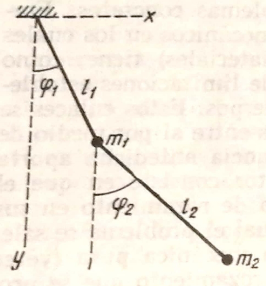
\includegraphics[width=0.3\textwidth]{img/pregunta_1.png}
  \caption{Péndulo Doble}
  \label{fig:pregunta_1}
\end{figure}

En este caso, tenemos $3 \cdot N = 3\cdot 2 = 6$ coordenadas cartesianas. Sin embargo, tenemos las siguientes ligaduras:
\begin{enumerate}
  \item $z = 0$
  \item  $l_1 = cte$
  \item $l_2 = cte$
\end{enumerate}

Por lo cual tenemos $3N - n = 3 \cdot 2 - 4 = 2$. Por lo tanto tenemos dos grados de libertad. Con esto entonces definamos las coordenadas generalizadas de la manera en la que nos propone la imagen \ref{fig:pregunta_1}. Con lo cual nos queda:
\begin{align*}
  x_1 &= l_1\cdot \sin\left(\varphi_1\right)  \implies \dot{x_1} = l_1 \dot{\varphi_1} \cos\left( \varphi_1 \right) \\
  y_1 &= -l_1\cdot \cos\left(\varphi_1\right) \implies \dot{y_1} = l_1\dot{\varphi_1}\sin\left( \varphi_1 \right) 
.\end{align*}

Dado que este primer caso es esencialmente un triangulo en donde estamos calculando los dos catetos (Note que el valor de $y$ es negativo)

Ahora bien, de manera similar, para la masa 2 esto seria como calcular estos mismos catetos. Sin embargo, debe iniciar desde los valores de $m_1$
\begin{align*}
  x_2 &= l_1\cdot \sin\left(\varphi_1\right) + l_2 \cdot \sin\left( \varphi_2 \right) \implies \dot{x_2} = l_1\dot{\varphi_1}\cos\left( \varphi_1 \right) + l_2 \dot{\varphi_2}\cos\left( \varphi_2 \right)  \\
  y_2 &= -l_1\cdot \cos\left(\varphi_1\right) - l_2 \cdot \cos\left( \varphi_2 \right) \implies \dot{y_2} = l_1\dot{\varphi_1}\sin\left( \varphi_1 \right) + l_2 \dot{\varphi_2}\sin\left( \varphi_2 \right)  \\
.\end{align*}

Con esto entonces, podemos calcular la energía cinética que es:
\begin{align*}
  T_1 &= \frac{1}{2}m_1v_1^2 \\
      &= \frac{1}{2}m_1\left( \dot{x}_1^2 + \dot{y}_1^2 \right)  \\
      &= \frac{1}{2}m_1\left( l_1^2\dot{\varphi_1}^2\cos^2\left( \varphi_1 \right) + l_1^2\dot{\varphi_1}^2 \sin^2\left( \varphi \right)  \right)  \\
      &= \frac{1}{2}m_1\left( l_1^2\dot{\varphi_1}^2 \right)\left( \cos^2\left( \varphi_1 \right) + \sin^2\left( \varphi_1 \right)  \right)   \\
      &= \frac{1}{2}m_1\left( l_1^2\dot{\varphi_1}^2 \right)
.\end{align*}

Y
\begin{align*}
  T_2 &= \frac{1}{2}m_2v_2^2 \\
      &= \frac{1}{2}m_2\left( \dot{x}_2^2 + \dot{y}_2^2 \right)  \\
      &= \frac{1}{2}m_2 \left( \left( l_1\dot{\varphi_1}\cos\left( \varphi_1 \right) + l_2 \dot{\varphi_2}\cos\left( \varphi_2 \right) \right)^2 + \left( l_1\dot{\varphi_1}\sin\left( \varphi_1 \right) + l_2 \dot{\varphi_2}\sin\left( \varphi_2 \right) \right)^2  \right)  \\
  \left( l_1\dot{\varphi_1}\cos\left( \varphi_1 \right) + l_2\dot{\varphi_2}\cos\left( \varphi_2 \right)  \right)^2 &= l_1^2\dot{\varphi_1}^2\cos^2\left( \varphi_1 \right) + 2l_1l_2\dot{\varphi_1}\dot{\varphi_2}\cos\left( \varphi_1 \right)\cos\left( \varphi_2 \right) + l_2^2\dot{\varphi_2}^2\cos^2\left( \varphi_2 \right)  \\
  \left( l_1\dot{\varphi_1}\sin\left( \varphi_1 \right) + l_2\dot{\varphi_2}\sin\left( \varphi_2 \right)  \right)^2 &= l_1^2\dot{\varphi_1}^2\sin^2\left( \varphi_1 \right) + 2l_1l_2\dot{\varphi_1}\dot{\varphi_2}\sin\left( \varphi_1 \right)\sin\left( \varphi_2 \right) + l_2^2\dot{\varphi_2}^2\sin^2\left( \varphi_2 \right)  \\
  l_1^2\dot{\varphi_1}^2\sin^2\left( \varphi_1 \right) + l_1^2\dot{\varphi_1}^2\cos^2\left( \varphi_1 \right)^2 &= l_1^2\dot{\varphi_1}^2\left( \sin^2\left( \varphi_1 \right) + \cos^2\left( \varphi_1 \right)  \right)  \\
														&\implies l_1^2 \dot{\varphi_1}^2 \\
  l_2^2\dot{\varphi_2}^2\sin^2\left( \varphi_2 \right) + l_2^2\dot{\varphi_2}^2\cos^2\left( \varphi_2 \right)^2 &= l_2^2\dot{\varphi_2}^2\left( \sin^2\left( \varphi_2 \right) + \cos^2\left( \varphi_2 \right)  \right)  \\
														&\implies l_2^2\dot{\varphi_2}^2 \\
  2l_1l_2\dot{\varphi_1}\dot{\varphi_2}\cos\left( \varphi_1 \right)\cos\left( \varphi_2 \right) &+ 2l_1l_2\dot{\varphi_1}\dot{\varphi_2}\sin\left( \varphi_1 \right)\sin\left( \varphi_2 \right) = 2l_1l_2\dot{\varphi_1}\dot{\varphi_2}\left( \cos\left( \varphi_1 \right)\cos\left( \varphi_2 \right) + \sin\left( \varphi_1 \right)\sin\left( \varphi_2 \right)  \right) \\
												&\implies 2l_1l_2\dot{\varphi_1}\dot{\varphi_2}\cos\left( \varphi_1 - \varphi_2 \right)  \\
												&= \frac{1}{2}m_2\left( l_1^2\dot{\varphi_1}^2 + l_2^2\dot{\varphi_2}^2  + 2l_1l_2\dot{\varphi_1}\dot{\varphi_2}\cos\left( \varphi_1 - \varphi_2 \right)\right) 
.\end{align*}

Ahora bien, para el caso de la energía potencial tenemos
\begin{align*}
  V_1 &= m_1gy_1 \\
  &= -m_1gl_1\cos\left( \varphi_1 \right)  \\
  V_2 &= m_2g y_2 \\
  &= -m_2g\left( l_1\cos\left( \varphi_{1} \right) + l_2\cos\left( \varphi_2 \right)  \right) 
.\end{align*}

Ahora bien, tenemos entonces que:
\begin{align*}
  T &= T_1 + T_2 \\
    &= \frac{1}{2}m_1\left( l_1^2\dot{\varphi}_1^2 \right) + \frac{1}{2}m_2\left( l_1^2\dot{\varphi_1}^2 + l_2^2\dot{\varphi_2}^2  + 2l_1l_2\dot{\varphi_1}\dot{\varphi_2}\cos\left( \varphi_1 - \varphi_2 \right)\right) \\
    &= \frac{1}{2}l_1^2\dot{\phi_1}^2\left( m_1 + m_2 \right) + \frac{1}{2}m_2l_2^2\dot{\phi_2}^2 + m_2l_1l_2\dot{\varphi_1}\dot{\varphi_2}\cos\left( \varphi_1 - \varphi_2 \right) 
.\end{align*}

Y
\begin{align*}
  V &= V_1 + V_2 \\
  &= -m_1gl_1\cos\left( \varphi_1 \right) -m_2gl_1\cos\left( \varphi_1 \right) - m_2gl_2\cos\left( \varphi_2 \right)  \\
  &= - gl_1\cos\left( \varphi_1 \right) \left( m_1 + m_2 \right) - m_2 gl_2\cos\left( \varphi_2 \right)
.\end{align*}

Por lo tanto dado que $L = T - V$ nos queda:
\begin{align*}
  L &= T - V \\
  L &=  \frac{1}{2}l_1^2\dot{\phi_1}^2\left( m_1 + m_2 \right) + \frac{1}{2}m_2l_2^2\dot{\phi_2}^2 + m_2l_1l_2\dot{\varphi_1}\dot{\varphi_2}\cos\left( \varphi_1 - \varphi_2 \right) -\left( - gl_1\cos\left( \varphi_1 \right) \left( m_1 + m_2 \right) - m_2 gl_2\cos\left( \varphi_2 \right) \right)  \\
   &=  \frac{1}{2}l_1^2\dot{\phi_1}^2\left( m_1 + m_2 \right) + \frac{1}{2}m_2l_2^2\dot{\phi_2}^2 + m_2l_1l_2\dot{\varphi_1}\dot{\varphi_2}\cos\left( \varphi_1 - \varphi_2 \right) +  gl_1\cos\left( \varphi_1 \right) \left( m_1 + m_2 \right) + m_2 gl_2\cos\left( \varphi_2 \right)
.\end{align*}

%%%%%%%%%%%%%%%%%%%%%%%%%%%%%%%%%%%%%%%%%%%%%%%%%%%%%%%%%%%%%%%%%%%%%%%%%%%%%%%%%%%%%%%%%%%%%%%%%%%%%%%%%%

\chapter{}

Quizás lo mejor en este caso es iniciar por notar que la altura del pivote depende de $L\cos\left( \theta \right) $ que es la altura dada por el angulo $\theta$ y también depende de $a\cos\left( \gamma t \right) $ que nos lo da el enunciado. Con esto entonces, podemos conseguir la energía potencial del sistema como: \[
V = - mg\left( a\cos\left( \gamma t \right) + L \cos\left( \theta \right)  \right) 
.\] Note que es negativo por que el sistema de coordenadas esta ordenado en ese sentido.

Una vez con esto, intentemos describir $T$ 
\begin{align*}
  T &= \frac{1}{2}m\left( \dot{x}^2 + \dot{y}^2 \right)  \\
    &= \frac{1}{2}m\left( L^2\cos^2\left( \theta \right)\dot{\theta} - \left(a\sin\left( \gamma t \right) + L \sin\left( \theta \right) \dot{\theta}\right)^2  \right)  \\
  \left(a\sin\left( \gamma t \right) + L \sin\left( \theta \right) \dot{\theta}\right)^2 &= a^2\sin^2\left( \gamma t \right) + a\sin\left( \gamma t \right) L\sin\left( \theta \right) \dot{\theta}  + L^2 \sin^2\left( \theta \right) \dot{\theta}^2\\
  L^2\cos^2\left( \theta \right) \dot{\theta}^2 - L^2\sin^2\left( \theta \right) \dot{\theta}^2 &= L^2\dot{\theta}^2 \\
												&= \frac{1}{2}m \left[ L^2\dot{\theta}^2 + a^2\gamma^2\sin^2\left( \gamma t \right) + 2 a\gamma\dot{\theta}L\sin\left( \gamma t \right) \sin\left( \theta \right)   \right]
.\end{align*}

Y con esto podemos encontrar el lagrangiano simplemente con
\begin{align*}
  \mathcal{L} &= T - V \\
  \mathcal{L} &=  \frac{1}{2}m \left[ L^2\dot{\theta}^2 + a^2\gamma^2\sin^2\left( \gamma t \right) + 2 a\gamma\dot{\theta}L\sin\left( \gamma t \right) \sin\left( \theta \right)   \right] + mg\left( a\cos\left( \gamma t \right) + L \cos\left( \theta \right)  \right)
.\end{align*}

%%%%%%%%%%%%%%%%%%%%%%%%%%%%%%%%%%%%%%%%%%%%%%%%%%%%%%%%%%%%%%%%%%%%%%%%%%%%%%%%%%%%%%%%%%%%%%%%%%%%%%%%%%
\chapter{}


\section{}

\subsection{}

Para comenzar, definamos cuantas coordenadas generalizadas existen. Dado que tenemos dos partículas tenemos $3N$ en coordenadas cartesianas. Ahora bien, tenemos 5 ligaduras las cuales son:
\begin{enumerate}
  \item $z_1 = 0$ 
  \item $z_2 = 0$ 
  \item 
    \begin{align*}
      \ell' &= \ell + \pi R\\
      \ell &= \ell' - \pi R \\
      \ell &= CTE\\
      \ell &= y_1 + y_2 = CTE
    .\end{align*}
  \item $x_1 = -R$
  \item $x_2 = R$
\end{enumerate}

Con esto entonces sabemos que tenemos $3N - n = 3\cdot 2 - 5 = 1$ grados de libertad. Por lo cual solo lo describiremos como $\phi$. En particular, tendremos que 
\begin{align*}
  y_1 &= \phi \\
  y_2 &= \ell - \phi
.\end{align*}

Una vez definimos esto, podemos calcular el lagrangiano:
\begin{align*}
  T &= \frac{1}{2}m_1\left( \dot{\phi} \right)^2 + \frac{1}{2}m_2\left( \dot{\phi} \right)^2 \\ V &= m_1g\phi + m_2g\left( \ell - \phi \right)  \\
  \mathcal{L} &= T - V \\
  &= \frac{1}{2}m_1\left( \dot{\phi} \right)^2 + \frac{1}{2}m_2\left( \dot{\phi} \right)^2 - \left( m_1g\phi + m_2g\left(\ell-\phi\right)\right)\\
  &= \left( \frac{1}{2}\dot{\phi}^2 \right)\left( m_1 + m_2 \right) - g\left(m_1\phi+m_2\ell-m_2\phi \right)
.\end{align*}

Con lo cual podemos mirar las ecuaciones de movimiento:
\begin{align*}
  \frac{\delta \mathcal{L}}{\delta \phi} &= 0 \\
  \frac{d}{dt}\left( \frac{\partial \mathcal{L}}{\partial \dot{\phi}}  \right) - \frac{\partial \mathcal{L}}{\partial \phi} &= 0 \\
  \frac{\partial \mathcal{L}}{\partial \dot{\phi}} &= \frac{\partial}{\partial \dot{\phi}} \left( \frac{1}{2}\dot{\phi}^2 \right)\left( m_1 + m_2 \right) - g\left( m_1\phi + m_2\ell - m_2\phi \right) \\
						   &= \left( m_1 + m_2 \right) \dot{\phi} \\
  \frac{d}{dt}\left( \frac{\partial \mathcal{L}}{\partial \phi}  \right) &= \frac{d}{dt}\left( \left( m_1 + m_2 \right)\dot{\phi}  \right)  \\
									 &= \left( m_1 + m_2 \right) \ddot{\phi} \\
  \frac{\partial \mathcal{L}}{\partial \phi} &= \frac{\partial}{\partial \phi} \left(\left( \frac{1}{2}\dot{\phi}^2 \right)\left( m_1 + m_2 \right) - g\left( m_1\phi + m_2\ell - m_2\phi \right)  \right)  \\
  &= -g\left( m_1 - m_2 \right)  \\
  \frac{d}{dt}\left( \frac{\partial \mathcal{L}}{\partial \dot{\phi}}  \right) - \frac{\partial \mathcal{L}}{\partial \phi} &= \left( m_1 + m_2 \right) \ddot{\phi} - \left( -g\left( m_1 - m_2 \right) \right) = 0 \\
  \left( m_1 + m_2 \right) \ddot{\phi} - \left( g\left( m_2 - m_1 \right) \right) &= 0\\
  \left( m_1 + m_2 \right) \ddot{\phi} &= g\left( m_2 - m_1 \right)  \\
  \ddot{\phi} &= \frac{g\left( m_2 - m_1 \right) }{\left( m_1 + m_2 \right) }
.\end{align*}

Sin embargo, esto no es en si mismo lo que nos pedía el ejercicio. Para esto debemos romper una ligadura pues como se ve la tensión no tendría sentido para este caso. En ese caso romperemos la ligadura de 3 o $\ell = CTE$. El procedimiento aunque no igual es semejante a medir la tensión con un dinamómetro. Con lo cual tendríamos: \[
\frac{\delta T}{\delta x} = Q_x \land \frac{\delta T}{\delta \ell} = Q_{\ell}
.\] Con lo cual
\begin{align*}
  \delta \omega &= \left( m_1g - \tau \right) \delta x + \left(m_2g=\tau\right)\left(-\delta x \right)  \\
  \delta \omega &= \left( m_1 - m_2 \right) g \delta x = Q_x \delta x \\
  Q_x &= \left( m_1 - m_2 \right)g
.\end{align*}

Ahora bien, dejando $x$ constante y variando $\ell$ entonces nos queda
\begin{align*}
  \delta \omega &= \left( m_2g - \tau \right)\delta \ell = Q_\ell d_\ell \\
  Q_\ell &= \left( m_2g - \tau \right)
.\end{align*}

Ahora bien, dado que lo que estamos variando es $\ell$ entonces nos queda:
\begin{align*}
  \dot{x}_2 &= \frac{dx_2}{dt} \\
  &= \frac{d}{dt}\left( \ell - x_1 \right)  \\
  &= \frac{d\ell}{dt} - \frac{d\ell}{dt} \\
  &= \dot{\ell} - \dot{x_1}
.\end{align*}

Con lo cual podemos ponerlo en $T$ 
\begin{align*}
  T &= \frac{1}{2}m_1\dot{x_1}^2 + \frac{1}{2}m_2\left( \dot{\ell} - \dot{x_1} \right)^2
.\end{align*}

Y ahora con esto entonces podemos volver a las ecuaciones de segundo orden
\begin{align*}
  \frac{\delta T}{\delta x} &= Q_x \\
  \frac{d}{dt}\left( \frac{\partial T}{\partial \dot{x_1}}  \right) - \frac{\partial T}{\partial x_1} &= Q_{x_1} \\
  \frac{\partial T}{\partial \dot{x}}&=m_1\dot{x_1}+m_2\left( \dot{\ell} - \dot{x} \right) \left( -1\right)\\
  \frac{\partial T}{\partial x}  &= 0 \\
  \frac{d}{dt}\left( \frac{\partial T}{\partial \dot{x}}  \right) &= m_1\ddot{x_1} - m_2\left( \ddot{\ell} - \ddot{x_1} \right)  \\
								  &= \left( m_1 + m_2 \right) \ddot{x_1} \\
  \frac{\delta T}{\delta x} &= \frac{d}{dt}\left( \frac{\partial T}{\partial \dot{x}}  \right)  \\
			    &= \left( m_1 + m_2 \right) \ddot{x_1}
.\end{align*}

Y por el otro lado
\begin{align*}
  \frac{\delta T}{\delta \ell} &= Q_\ell \\
  \frac{d}{dt}\left( \frac{\partial T}{\partial \dot{\ell}}  \right) - \frac{\partial T}{\partial \ell} &= Q_\ell \\
  \frac{\partial T}{\partial \dot{\ell}} &= m_2\left( \dot{\ell} - \dot{x_1} \right)  \\
  \frac{d}{dt}\left( \frac{\partial T}{\partial \dot{\ell}}  \right) &= m_2 \ddot{\ell} - m_2\ddot{x_1} \\
  \frac{\partial T}{\partial \ell} &= 0 \\
  \frac{\delta T}{\delta \ell} &= \frac{d}{dt}\left( \frac{\partial T}{\partial \dot{\ell}}  \right) - \frac{\partial T}{\partial \ell}  \\
			       &= -m_2\ddot{x_1} = Q_\ell \\
			       &= m_2g - \tau
.\end{align*}

Con lo cual tendríamos
\begin{align*}
  \tau &= m_2\ddot{x_1} + m_2g \\
       &= m_2\left( \ddot{x_1} + g \right)  \\
       &= m_2\left( g + \frac{\left( m_1 - m_2 \right) }{\left( m_1 + m_2 \right) }g \right)  \\
       &= m_2\left( \frac{g\left( m_1 - m_2 \right) + g\left( m_1 + m_2 \right) }{m_1 + m_2} \right)  \\
       &= \frac{2m_1m_2 g}{m_1 + m_2}
.\end{align*}

\subsection{}

Ahora con multiplicadores de Lagrange tendríamos dos coordenadas generalizadas y por tanto esto quedaría:
\begin{align*}
  \frac{\delta \mathcal{L}}{\delta q_i} &= \frac{d}{dt}\left( \frac{\partial \mathcal{L}}{\partial \dot{q_i}}  \right) - \left( \frac{\partial \mathcal{L}}{\partial q_i}  \right) = \sum_{n=1}^{2} \lambda_n \frac{\partial F_n}{\partial q_n} = Q \\
  \mathcal{L} &= T - V \\
  \mathcal{L} &= \left( \frac{1}{2}m_1\dot{x_1}^2 + \frac{1}{2}m_2\dot{x_2}^2 \right) - \left( m_1gx_1 + m_2gx_2 \right) 
\end{align*}

Con este lagrangiano podemos obtener

\begin{align*}
  \frac{\partial \mathcal{L}}{\partial \dot{q_1}} &= m_1\dot{x_1}\\
  \frac{d}{dt}\left( \frac{\partial \mathcal{L}}{\partial \dot{q_1}}  \right) &= m_1\ddot{x_1}\\
  \frac{\partial \mathcal{L}}{\partial q_1} &= -m_1g \\
  \frac{\delta \mathcal{L}}{\delta q_1} &= m_1\ddot{x_1} + m_1g = \lambda \frac{\partial F}{\partial q_1} = \lambda
.\end{align*}

Igual que para $q_2$ 
\begin{align*}
  \frac{\partial \mathcal{L}}{\partial \dot{q_2}} &= m_2\dot{x_2} \\
  \frac{d}{dt}\frac{\partial \mathcal{L}}{\partial \dot{q_2}} = m_2\ddot{x_2}\\
  \frac{\partial \mathcal{L}}{\partial q_2} &= -m_2g \\
  \frac{\delta \mathcal{L}}{\delta q_2} &= m_2\ddot{x_2} + m_2g = \lambda \frac{\partial F}{\partial x_2} = \lambda
.\end{align*}

Con esto entonces podemos desarrollar
\begin{align*}
  m_1\ddot{x_1} + m_1g &= \lambda \\
  m_2\ddot{x_2} + m_2g &= \lambda \\
  F &= x_1 + x_2 \\
  m_1\ddot{x_1} + m_1 g &= m_2\ddot{x_2} + m_2g \\
  m_1\left( - \ddot{x_2} \right) - m_2 \ddot{x_2} &= m_2g - m_1g  \\
  -\ddot{x_2}\left( m_1 + m_2 \right) &= g \left( m_2 - m_1 \right)  \\
  -\ddot{x_2} &= \frac{g\left( m_2 - m_1 \right) }{m_1 + m_2} \\
  \ddot{x_1} &= \frac{g\left( m_2 - m_1 \right) }{\left( m_1 + m_2 \right) }
.\end{align*}

Que ahora con la primera ecuación nos queda: \[
  \lambda = m_1\left( \ddot{x_1} + g \right)
.\] 

Ahora podemos desarrollar la tensión como
\begin{align*}
       \tau &= m_1\left( g + \frac{\left( m_2 - m_1 \right) }{\left( m_1 + m_2 \right) }g \right)  \\
       &= m_1\left( \frac{g\left( m_2 - m_1 \right) + g\left( m_1 + m_2 \right) }{m_1 + m_2} \right)  \\
       &= \frac{2m_1m_2 g}{m_1 + m_2}
.\end{align*}

\section{}

Con esta cuenta, lo que podemos hacer es definir unas coordenadas generalizadas que sean solo el radio en el que se encuentra la cuenta respecto al eje desde donde ocurre la rotación. Por lo tanto, esto lo podemos expresar como:
\begin{align*}
  x = r\cos\left( \dot{\theta}t \right) \implies \dot{x} = \dot{r}\cos\left( \dot{\theta}t \right) - r\dot{\theta}\sin\left( \dot{\theta}t \right) \\
  y = r\sin\left( \dot{\theta} \right)  \implies \dot{y} = \dot{r}\sin\left( \dot{\theta}t \right) + r\dot{\theta}\cos\left( \dot{\theta}t \right) 
.\end{align*}

Ahora bien, dado que esta cuenta se esta moviendo solamente y no tenemos efectos de otras fuerzas entonces este sistema no tiene energía potencial. Por lo tanto solo necesitamos la energía cinética para encontrar el lagrangiano.

\begin{align*}
  T &= \frac{1}{2}m\left[ \left( \dot{r}\cos\left( \dot{\theta}t \right) - r\dot{\theta}\sin\left( \dot{\theta}t \right) \right)^2 + \left( \dot{r}\sin\left( \dot{\theta}t \right) + r\dot{\theta}\cos\left( \dot{\theta}t \right) \right)^2  \right] \\
  \left( \dot{r}\cos\left( \dot{\theta}t \right) - r\dot{\theta}\sin\left( \dot{\theta}t \right) \right)^2 &= \dot{r}^2\cos^2\left( \dot{\theta}t \right) - 2\dot{r}r\dot{\theta}\cos\left( \dot{\theta}t \right)\sin\left( \dot{\theta}t \right)  + r^2\dot{\theta}^2\sin^2\left( \dot{\theta}t \right) \\
  \left( \dot{r}\sin\left( \dot{\theta}t \right) - r\dot{\theta}\cos\left( \dot{\theta}t \right) \right)^2 &= \dot{r}^2\sin^2\left( \dot{\theta}t \right) + 2\dot{r}r\dot{\theta}\sin\left( \dot{\theta}t \right)\cos\left( \dot{\theta}t \right)  + r^2\dot{\theta}^2\cos^2\left( \dot{\theta}t \right) \\
  \dot{r}^2\sin^2\left( \dot{\theta}t \right) + \dot{r}^2\cos^2\left( \dot{\theta}t \right) &= \dot{r}^2\left( \cos^2\left( \dot{\theta}t \right) + \sin^2\left( \dot{\theta}t \right)  \right)  \\
											    &\implies \dot{r}^2\\
											    2\dot{r}r\dot{\theta}\cos\left( \dot{\theta}t \right)\sin\left( \dot{\theta}t \right) - 2\dot{r}r\dot{\theta}\cos\left( \dot{\theta}t \right)\sin\left( \dot{\theta}t \right) &= 0 \\
											    r^2\dot{\theta}^2\cos^2\left( \dot{\theta}t \right) + r^2\dot{\theta}^2\cos^2\left( \dot{\theta}t \right) &= r^2\dot{\theta}^2 \left( \cos^2\left( \dot{\theta}t \right) + \sin^2\left( \dot{\theta}t \right)  \right)  \\
																								      &\implies r^2\dot{\theta}^2\\
											    T &= \frac{1}{2}m\left(\dot{r}^2 + r^2\dot{\theta}^2 \right) = \mathcal{L}
.\end{align*}

Ahora con esto:
\begin{align*}
  \frac{\partial \mathcal{L}}{\partial r} &= mr\dot{\theta}^2 \\
  \frac{\partial \mathcal{L}}{\partial \dot{r}} &= m\dot{r}\\
  \frac{d}{dt}\left( \frac{\partial \mathcal{L}}{\partial r}  \right) &= m \ddot{r} \\
  m\ddot{r} - mr\dot{\theta}^2 &= 0 \\
  \ddot{r} - r\dot{\theta}^2 &= 0 \\
  r &= \dot{\theta}^2
.\end{align*}


%%%%%%%%%%%%%%%%%%%%%%%%%%%%%%%%%%%%%%%%%%%%%%%%%%%%%%%%%%%%%%%%%%%%%%%%%%%%%%%%%%%%%%%%%%%%%%%%%%%%%%%%%%
\chapter{}

En este caso vamos a partir de que un cilindro rueda sobre otro. Para este caso tenemos dos cilindros, uno de radio $a$  y uno de radio $\alpha a$. Las medidas se pueden observar en la figura \ref{fig:img-pregunta_3_1-png}. 

\begin{figure}[H]
  \centering
  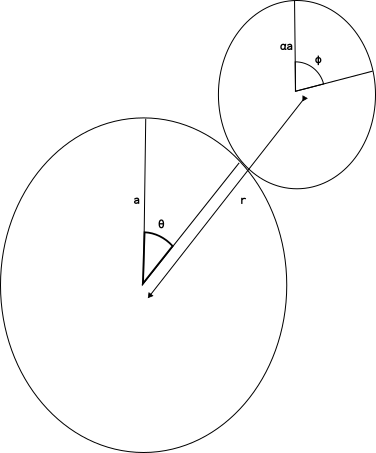
\includegraphics[width=0.4\textwidth]{img/pregunta_3_1.png}
  \caption{Dimensiones y descripción del problema}
  \label{fig:img-pregunta_3_1-png}
\end{figure}

Con esto entonces nos hace falta ver las fuerzas que las puede encontrar en la figura \ref{fig:img-pregunta_3_2-png}

\begin{figure}[H]
  \centering
  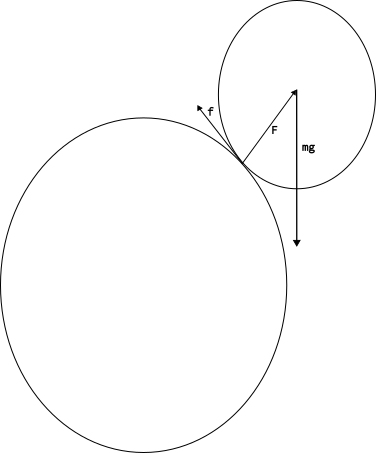
\includegraphics[width=0.4\textwidth]{img/pregunta_3_2.png}
  \caption{Fuerzas en el sistema}
  \label{fig:img-pregunta_3_2-png}
\end{figure}

En este caso, dado que el cilindro $\alpha a$ ira teniendo cada vez una menor fuerza $Z$ (dado que el angulo en el que se encuentra con respecto a su eje disminuye) entonces sabemos que eventualmente este cilindro se despegara del fijo $a$. Ademas, sabemos que estos dos perderán contacto en cuanto la fuerza normal  $F$ ya no tenga ingerencia. Es decir, cuando \[
F = 0
.\] Ademas, sabemos por el como funciona la fricción que \[
f \le \mu F
.\] donde $\mu$ es el coeficiente de fricción. Lo que implica que este movimiento eventualmente empezara a deslizar sobre la superficie. Por lo tanto, podemos dividir este análisis en 3 momentos definidos por los ángulos $\theta_1$, $\theta_2$ y $\theta_3$. Para iniciar, desde $0$ hasta $\theta_1$ el cilindro rueda sin deslizar, lo que se describe en que la fricción seria \[
f = \mu F
.\] Ahora, entre $\theta_1$ y $\theta_2$ el cilindro se deslizaría pues la fricción es muy pequeña y en $\theta_2$ el cilindro dejaría de estar en contacto con el otro y por lo tanto se sostendría $F = 0$ y de ahí en adelante caería libremente.

Ahora bien iniciemos caso a caso
\section{}

Para empezar para un movimiento que no desliza entonces sabemos que:
\begin{align*}
  a\theta &= \alpha a \left( \varphi - \theta \right) \\
  \theta &= \alpha \left( \varphi - \theta \right) \\
  \theta &= \alpha \varphi - \alpha \theta \\
  \theta + \alpha \theta &= \alpha\varphi \\
  \left( 1 + \alpha \right) \theta &= \alpha \varphi
.\end{align*}

Ahora bien, podemos definir una función desarrollando:
\begin{align*}
  \left( 1 + \alpha \right) \theta &= \alpha \varphi \\
  \theta &= \frac{\alpha \varphi}{\left( 1 + \alpha \right) } \\
  \gamma &= \theta - \frac{\alpha \varphi}{\left( 1 + \alpha \right) }\\
  \frac{\alpha \varphi}{\left( 1 + \alpha \right) } &= \theta - \gamma \\
  \alpha \varphi &= \left( \theta - \gamma \right) \left( 1 + \alpha \right)  \\
  \varphi &= \frac{\left( \theta - \gamma \right) \left( 1 + \alpha \right) }{\alpha}
.\end{align*}

Donde, como se puede notar cuando esto no desliza $\gamma = 0$. Ahora bien, por otro lado, tenemos que al estar estos dos cilindros en contacto la distancia entre los centros queda: \[
r = a + \alpha a = \left( 1 + \alpha \right) a
.\] Ahora bien,
\begin{align*}
  T &= \frac{1}{2}m\left( \dot{r}^2 + r^2\dot{\theta}^2 \right) + \frac{1}{2}\left( \frac{1}{2}m \right) \left( \alpha^2 a^2 \dot{\varphi}^2 \right)  \\
    &= \frac{1}{2}m\dot{r}^2 + \frac{1}{2}m r^2\dot{\theta}^2 + \frac{1}{4}m\left( \alpha^2 a^2 \left( \frac{\left( \theta - \gamma \right)\left( 1 + \alpha \right) }{\alpha} \right)^2 \right) \\ 
    \frac{1}{4} m \left( \alpha^2 a^2 \left( \frac{\left( \theta - \gamma \right) \left( 1 + \alpha \right) }{\alpha} \right)^2 \right) &= \frac{1}{4}m \left( \alpha^2 a^2 \frac{\left( \theta - \gamma \right)^2 \left( 1 + \alpha \right)^2}{\alpha^2} \right)  \\
    &=  \frac{1}{4}m \left( a^2 \left( 1 + \alpha \right)^2 \left( \dot{\theta}^2 - 2\dot{\gamma}\dot{\theta} + \dot{\gamma}^2 \right)  \right) \\
    T &= \frac{1}{2}m\dot{r}^2 + \frac{1}{2}m r^2\dot{\theta}^2 +\frac{1}{4}m \left( a^2 \left( 1 + \alpha \right)^2 \left( \dot{\theta}^2 - 2\dot{\gamma}\dot{\theta} + \dot{\gamma}^2 \right)  \right)
.\end{align*}

Ahora bien, podemos encontrar las fuerzas generalizadas con la ecuación
\begin{align*}
  \delta W_k &= Q_k \delta q_k \\
  Q_k &= \frac{\delta W_k}{\delta q_k} \\
  Q_k &= - \frac{\partial V}{\partial q_k}
.\end{align*}

Con lo cual, podríamos usar:
\begin{align*}
  V &= mgr\cos\left( \theta \right) + \gamma fa\left( 1 + \alpha \right) - F_r  \\
  Q_k &= - \frac{\partial V}{\partial k}  \\
  Q_\theta &= - \left( - mgr \sin\left( \theta \right) + 0 + 0 \right)  \\
  &= mgr \sin\left( \theta \right)  \\
  Q_\gamma &= - \left( 0 + f\left( 1 + \alpha \right) - 0 \right)  \\
  &= -fa\left( 1 + \alpha \right)  \\
  Q_r &= - \left( mg\cos\left( \theta \right) - F\right)  \\
  &= F - mg\cos\left( \theta \right)
.\end{align*}

Con lo cual

\begin{align*}
  Q_\theta &= mgr\sin\left( \theta \right)  \\
  Q_\gamma &= - fa\left( 1 + \alpha \right)  \\
  Q_r &= F - mg\cos\left( \theta \right)
.\end{align*}

Ahora bien, queda:
\begin{align*}
  \mathcal{L} &= T - V \\
  &=  \frac{1}{2}m\dot{r}^2 + \frac{1}{2}m r^2\dot{\theta}^2 +\frac{1}{4}m \left( a^2 \left( 1 + \alpha \right)^2 \left( \dot{\theta}^2 - 2\dot{\gamma}\dot{\theta} + \dot{\gamma}^2 \right)  \right)\\
  &- \left( mgr\cos\left( \theta \right) + \gamma fa\left( 1 + \alpha \right) - Fr \right) 
.\end{align*}

Con lo cual \[
  \frac{d}{dt}\left( \frac{\partial \mathcal{L}}{\partial \dot{q_k}}  \right) - \frac{\partial \mathcal{L}}{\partial q_k} = Q_k
.\] 

Ahora para esto:
\begin{align*}
  \frac{\partial \mathcal{L}}{\partial \theta} &= mr^2\dot{\theta} + \frac{1}{2}m\left( a^2\left( 1 + \alpha \right)^2 \right)\left( \dot{\theta} - \dot{\gamma} \right)  \\
.\end{align*}

%%%%%%%%%%%%%%%%%%%%%%%%%%%%%%%%%%%%%%%%%%%%%%%%%%%%%%%%%%%%%%%%%%%%%%%%%%%%%%%%%%%%%%%%%%%%%%%%%%%%%%%%%%

\chapter{}

Dado que estamos en un péndulo esférico lo mas simple es pasar nuestras coordenadas generalizadas para que sean esféricas. En este caso, las velocidades son:
\begin{align*}
  \dot{r}^2 + r^2\dot{\theta}^2 + r^2\dot{\ell}^2\sin^2\left( \theta \right) 
.\end{align*}

Ahora bien, dado que este es un péndulo sabemos que $r$ es constante. Por lo tanto, mis coordenadas generalizadas serian $\theta$ y $\ell$. Y con la velocidad descrita como arriba la energía cinética me queda como:
\begin{align*}
  T &= \frac{1}{2}m\left( r^2\dot{\theta}^2 + r^2\dot{\ell}^2\sin^2\left( \theta \right)  \right)  \\
.\end{align*}

Por otro lado, el único potencial que existe en este sistema es el gravitacional  y este solo depende de $\theta$ dado que solo esta definido por la altura. Por lo tanto este queda como \[
V = mg r\cos\left( \theta \right) 
.\] Con esto ya calculado podemos saber que el lagrangiano es
\begin{align*}
  \mathcal{L} = T - V = \frac{1}{2}m\left( r^2\dot{\theta}^2 + r^2\dot{\ell}^2\sin^2\left( \theta \right)  \right) - mgr\cos\left( \theta \right) 
.\end{align*}

Con esto entonces las ecuaciones de Euler Lagrange nos quedan como
\begin{align*}
  \frac{\delta \mathcal{L}}{\delta \theta} &= 0 \\
  \frac{\partial \mathcal{L}}{\partial \dot{\theta}} &= mr^2\dot{\theta} \\
  \frac{d}{dt}\frac{\partial \mathcal{L}}{\partial \dot{\theta}} &= m\ddot{\theta}r^2 \\
  \frac{\partial \mathcal{L}}{\partial \theta} &= mr^2\dot{\ell}^2\sin\left( \theta \right) \cos\left( \theta \right) + mgr\sin\left( \theta \right)  \\
  \frac{\delta \mathcal{L}}{\delta \theta} &= mr^2\ddot{\theta} -mr^2\dot{\ell}^2\sin\left( \theta \right) \cos\left( \theta \right) - mgr\sin\left( \theta \right) = 0 \\
  \frac{\delta \mathcal{L}}{\delta \ell} &= 0 \\
  \frac{\partial \mathcal{L}}{\partial \dot{\ell}} &= mr^2\dot{\ell}\sin^2\left( \theta \right)  \\
  \frac{d}{dt}\frac{\partial \mathcal{L}}{\partial \dot{\ell}} &= mr^2\ddot{\ell}\sin^2\left( \theta \right) \\
  \frac{\partial \mathcal{L}}{\partial \ell} &= 0\\
  \frac{\delta \mathcal{L}}{\delta \ell} &= mr^2\ddot{\ell}\sin^2\left( \theta \right) = 0
.\end{align*}

Note que
\begin{align*}
  \frac{\delta \mathcal{L}}{\delta \ell} &= mr^2\ddot{\ell}\sin^2\left( \theta \right) = 0\\
  0 &= \frac{d}{dt}\left( mr^2\dot{\ell}\sin^2\left( \theta \right) \right)  \\
  p_\ell &= CTE =  mr^2\dot{\ell}\sin^2\left( \theta \right)
.\end{align*}

Ahora bien, sabemos que \[
  \dot{\theta} \frac{\partial L}{\partial \dot{\theta}} + \dot{\ell}\frac{\partial L}{\partial \dot{\ell}} - L = E
.\] donde $E$ es una constante, que al reemplazar todo nos queda como
\begin{align*}
  \frac{1}{2}mr^2\dot{\theta}^2 + \frac{p_\ell^{2}}{2mr^2\sin^2\left( \theta \right) } + mgr\cos\left( \theta \right) &= E \\
.\end{align*}

Con esto podemos tomar lo que esencialmente es un potencial en este caso como:
\begin{align*}
  \mathcal{V} = \frac{p_\ell^{2}}{2mr^2\sin^2\left( \theta \right) } + mgr\cos\left( \theta \right)
.\end{align*}

%%%%%%%%%%%%%%%%%%%%%%%%%%%%%%%%%%%%%%%%%%%%%%%%%%%%%%%%%%%%%%%%%%%%%%%%%%%%%%%%%%%%%%%%%%%%%%%%%%%%%%%%%%
\chapter{}

Para iniciar podemos describir la energía cinética como:
\begin{align*}
  T &= \frac{1}{2}mv^2 \\
  T &= \frac{1}{2}m\left( a^2\dot{\theta}^2 + a^2\omega^2 \sin^2\left( \theta \right)  \right)  \\
  T &= \frac{1}{2}ma^2\dot{\theta}^2 + \frac{1}{2}ma^2\omega^2\sin^2\left( \theta \right)  \\
  V &= -mgy\\
  V &= -mg\left( a \cos\left( \theta \right)  \right)  \\
  \mathcal{L} &= T - V \\
  \mathcal{L} &= \frac{1}{2}ma^2\dot{\theta}^2 + \frac{1}{2}ma^2\omega^2\sin^2\left( \theta \right) + mg\left( a \cos\left( \theta \right) \right) 
.\end{align*}

Ademas, podemos notar que \[
  \frac{\partial \mathcal{L}}{\partial t}  = 0
.\] Con esto entonces, podemos utilizar la ecuación: \[
\sum_{k=1}^{f} \dot{q_k}\frac{\partial \mathcal{L}}{\partial \dot{q_k}} - \mathcal{L} = CTE
.\] Que dado que solo tenemos un grado de libertad esto se puede resumir a

\begin{align*}
  \dot{q_k}\frac{\partial \mathcal{L}}{\partial \dot{q_k}} &= \left( ma^2\dot{\theta}^2 \right) -\frac{1}{2}ma^2\dot{\theta}^2 - \frac{1}{2}ma^2\omega^2\sin^2\left( \theta \right) - mg\left( a \cos\left( \theta \right) \right)   \\
  &= \frac{1}{2}ma^2\dot{\theta}^2 - \frac{1}{2}ma^2\omega^2\sin^2\left( \theta \right) - mg\left( a \cos\left( \theta \right) \right) \\
  &= \mathcal{E}
.\end{align*}

Que esto lo podemos tomar como un lagrangiano con un eje fijo. Con lo cual
\begin{align*}
  \mathcal{V}\left( \theta \right) &= -\frac{1}{2}ma^2\omega^2\sin^2\left( \theta \right) - mga\cos\left( \theta \right)  \\
.\end{align*}

Que para comprobar la velocidad angular limite tenemos
\begin{align*}
  \mathcal{V}\left( \theta \right) &= -\frac{1}{2}ma^2\omega^2\sin^2\left( \theta \right)  - mga\cos\left( \theta \right) \\
  &= -\frac{1}{2}ma^2\left( \left( \frac{g}{a} \right)^{\frac{1}{2}} \right)^2\sin^2\left( \theta \right)  - mga\cos\left( \theta \right)  \\
  &= -\frac{1}{2}mag\sin^2\left( \theta \right)  - mga\cos\left( \theta \right)  \\
  &= -\frac{1}{2}\sin^2\left( \theta \right) - \cos\left( \theta \right)  \\
.\end{align*}

\end{document}
